\section{Список смежности Ia}
\subsection{Условие задания}
\textbf{Вариант 20:} Вывести все вершины орграфа, не смежные с данной.

\subsection{Примеры исходного кода}
Для нахождения и вывода вершин орграфа, не смежных с данной, был
описан метод \mitext{getAdjacent()}:
\begin{minted}{typescript}
getAdjacent(label: string): Map<string, number> {
  if (!this.adj.has(label)) {
    throw new NodeNotExists(label)
  }
  return this.adj.get(label)!
}
\end{minted}

Затем, при выводе результата, запрашиваются все метки вершин орграфа и
из них отбрасываются те, которые смежны с данной:
\begin{minted}{typescript}
let resList: string[] = []
for (const [node, _] of graph.current!.getAdjacencyList()) {
  if (nodeName !== node && !adj.has(node)) {
    resList.push(node.toString())
  }
}
setAnswer(resList.join(', '))
\end{minted}

\subsection{Краткое описание алгоритма}
Поскольку данные о смежности хранятся в виде списка смежности, достаточно
для заданной вершины запросить информацию о смежных с ней вершинах.
А далее простая фильтрация списка строк.

Поскольку графы могут быть взвешенными, и как пересекать веса не оговаривается,
то выбирается минимум из двух весов при пересечении.

\subsection{Примеры входных и выходных данных}
\subsubsection{Входные данные}
\begin{figure}[H]
  \begin{minipage}{0.5\textwidth}
    \centering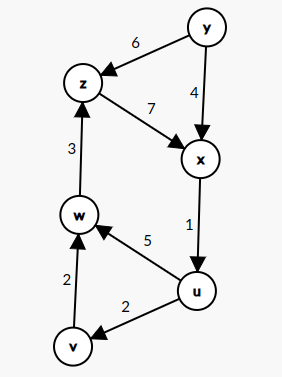
\includegraphics[width=0.6\linewidth]{figs/task-3/graph-2.png}
  \end{minipage}
  \begin{minipage}{0.5\textwidth}
    \centering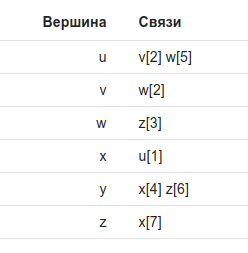
\includegraphics[width=0.6\linewidth]{figs/task-3/adj-2.png}
  \end{minipage}
  \caption{Ориентированный граф}
\end{figure}

\begin{minted}{js}
{
  "weighted": true,
  "oriented": true,
  "adj": {
    "u": {
      "v": 2,
      "w": 5
    },
    "v": {
      "w": 2
    },
    "w": {
      "z": 3
    },
    "x": {
      "u": 1
    },
    "y": {
      "x": 4,
      "z": 6
    },
    "z": {
      "x": 7
    }
  }
}
\end{minted}

\subsubsection{Выходные данные}
\begin{figure}[H]
  \centering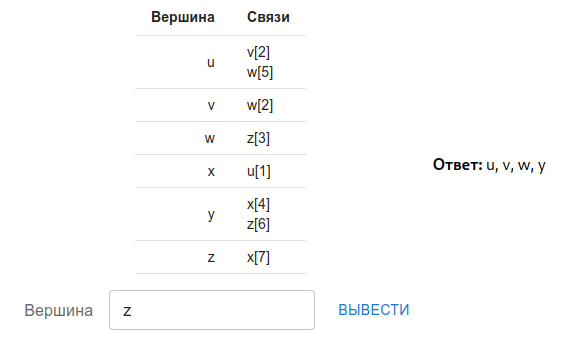
\includegraphics[width=0.8\textwidth]{figs/task-3/res-2.png}
  \caption{Результат работы}
\end{figure}